\Author{\daAuthorOne}

How can adaptive algorithms and real-time data integration be used to continuously update address databases and ensure accuracy in an app designed for mobile response teams?\\

Mobile field teams need address databases that stay up to date in real time. However, traditional methods cannot keep up with fast changes like road closures, new buildings or street name changes. Manual updates take time, and fixed validation rules do not account for regional differences or typos. These issues can lead to wasted time or even serious risks in critical situations.\\

This chapter explains how adaptive algorithms and real-time data integration can helkp solve these problems. Adaptive algorithms improve address databases by learning from new data, while real-time systems process live updates instantly. Together, they help mobile apps keep up with changing environments.



    \subsection{Traditional Methods for Address Database Management}

    Traditional address database management relies on manual or semi-automated processes that do not adapt in real time. These methods were created for stable environments with infrequent data changes, making them less effective for modern mobile applications that need constant updates. The following sections outline common challenges faced by traditional systems and their limitations in dynamic scenarios.

        \subsubsection{Manual Entry and Batch Updates}
        In the past, address databases were updated through periodic batch uploads, such as monthly CSV files, which store data in a table format with each value separated by commas. Organizations often relied on printed address lists provided to field teams, with corrections submitted on paper. This method caused delays. If a street name changed due to construction, mobile teams could work with outdated data for long time periods. \autocite{FasterCapital2025Mar}\\

        Manual data entry by administrators was another common practice. Human errors, such as typos, worsened the problem, making the system less reliable. A study conducted by the Journal of Accountancy found that human error rates in manual data entry can range from 1\% to 5\%. \autocite{integrationmadeeasy2025Mar}

        \subsubsection{Static Validation Rules}
        Many traditional systems rely on rigid validation rules, such as regular expressions, to verify address formats. Regex is a tool used to define patterns for strings, making it useful for matching specific formats. For example, a regex pattern might require the full word "Street" rather than abbreviations like "St." or "Str.".\autocite{AutorenderWikimedia-Projekte2002Jul}\\
        
        While this enforces consistency, it struggles to accommodate regional differences or new address formats. In some cases, a German address with "Straße" may pass validation, but an abbreviation like "Str." might be rejected, even though it is commonly used by field teams.


        \subsubsection{Third-Party Data Purchasing}
        Third-party data purchasing involves purchasing address datasets from external providers to update and maintain address information. These datasets are typically updated on a set schedule, such as quarterly, and are intended to offer broad coverage of geographic areas. However, the problem with this approach is that the data can become outdated quickly, especially in environments where changes occur rapidly. For example, temporary road closures, new constructions, or damage to infrastructure might not be reflected in the datasets if updates are infrequent. As a result, teams relying on outdated maps might encounter roads that are blocked or no longer accessible, which are not reflected in the datasets. This lack of real-time updates can cause delays in reaching critical locations, reduce the efficiency of field teams, and create potentially hazardous situations.



    \subsection{Adaptive Algorithms}
    Adaptive algorithms are methods that continuously adjust their parameters in response to new data and changing environmental conditions. These techniques are vital for applications where real-time adaptation is necessary. The following sections describe several core approaches within this domain.


        \subsubsection{Fuzzy Matching}
        Fuzzy Matching, also known as Approximate String Matching or Fuzzy Logic Name Matching, is a technique designed to find approximate matches between two pieces of data or text. It is commonly used in fields powered by Artificial Intelligence and Machine Learning.\\

        At its core, fuzzy matching is a string-matching algorithm that helps identify duplicate strings, words, or entries that closely resemble each other, even when there are abbreviations or misspellings. The technique works by applying edit operations such as insertion, deletion, substitution, and transposition to adjust the strings. These operations are measured in terms of an "editing distance," which influences the match score.\\
        
        Fuzzy matching is widely applied in various fields, such as document data extraction, spell-checking suggestions, deduplication, and even genome sequencing. It helps achieve high data accuracy by identifying and matching errors, ultimately keeping databases clean by detecting duplicates.\autocite{Nieters2024Dec}

        \begin{figure}[H]
            \centering
            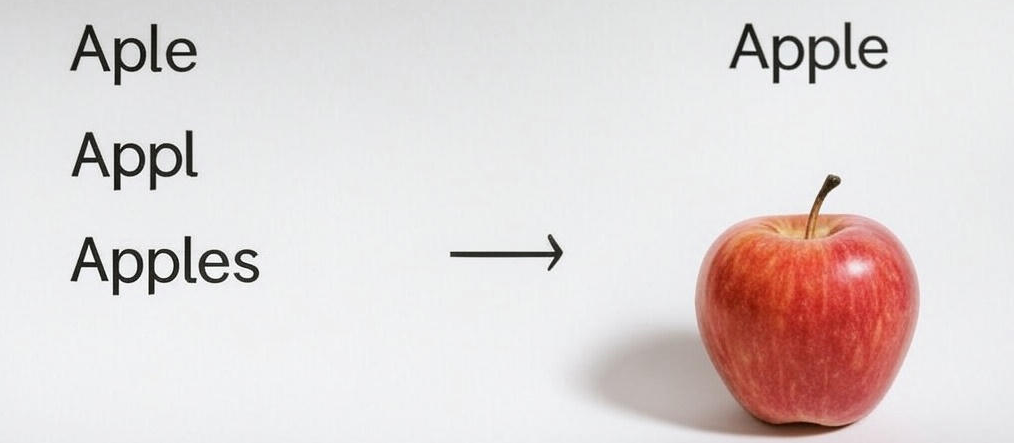
\includegraphics[width=0.5\textwidth]{images/AdminPanel/FuzzyMatching.png}
            \caption{Fuzzy Matching Example}
            \label{fig:fuzzy-matching}
        \end{figure}

        \subsubsection{Machine Learning Model}
        Incorporating machine learning models within adaptive systems allows for continuous improvement in prediction and classification tasks. These models, often designed to learn in an online or incremental fashion, update their parameters as new data streams in. This ongoing refinement enhances the system's ability to detect anomalies, forecast trends, and generate real-time recommendations. Ensemble techniques are sometimes used to combine multiple models, further increasing the robustness and accuracy of the overall system.

        \subsubsection{Rule-Based Filters}
        Rule-based filters are used to categorize and identify elements based on specific parameters or criteria, and they modify the visibility or graphical display of these elements when applied. For example, to change the line style and color of 2-hour fire-rated walls in a view, a rule-based filter is created to select all walls that have a 2-hour fire rating. The filter is then applied to the view, and its visibility and graphic settings, such as line style and color, are defined. As a result, all walls meeting the filter criteria will display according to the specified settings.\\

        A rule-based filter consists of one or more rule sets, and each rule set can contain multiple rules and/or nested rule sets. There is no limit to the number of rules or sets that can be defined. Rule sets use logical conditions like AND or OR:\\
        
        AND: All rules within the rule set must be true for the filter to apply.
        OR: At least one rule within the rule set must be true for the filter to apply.
        When creating a filter, the process involves:\\
        
        Selecting one or more categories to filter.
        Creating rule sets for each category.
        Defining parameters, operators, and values for each rule. The parameters depend on the categories chosen and can include instance, type, project, and shared parameters. If worksets are enabled, the Workset parameter is also available. Operators are selected based on the type of parameter, and values can be chosen from a drop-down list or manually entered. Text values are case-insensitive.
        \subsubsection{Dynamic Duplicate Resolution}
        When managing large, continuously updated datasets, resolving duplicate entries in real time becomes a critical challenge. Advanced duplicate resolution techniques combine similarity metrics and predictive modeling to continuously monitor data streams. The process involves detecting potential duplicates using fuzzy matching and then merging records based on contextual cues and historical data trends. This dynamic approach helps maintain a clean, unified dataset, which is especially important for applications like customer relationship management and large-scale data warehousing.


    \subsection{Real-Time Data Integration Frameworks}
    Real-time data integration frameworks are systems designed to collect, process, and deliver data instantly as it is generated. Unlike traditional batch processing, which handles data in chunks, these frameworks enable continuous updates. This makes them ideal for applications where delays are unacceptable. \textit{For mobile apps targeting field teams, such frameworks ensure that address databases stay accurate by integrating live data from multiple sources (e.g., GPS, user feedback, external APIs) without manual intervention.}

        \subsubsection{Challanges}
        Real-time data integration faces several hurdles, especially in dynamic environments like mobile field operations. First, \textbf{latency} can render updates useless for time-sensitive tasks. Emergency teams relying on outdated addresses risk missing critical locations. Frameworks address this with in-memory computing or edge computing. Second, \textbf{data quality} issues like typos or GPS drift require adaptive algorithms. \textit{For example, fuzzy matching (e.g., Levenshtein distance) corrects discrepancies on the fly}. Third, \textbf{scalability} is critical when handling thousands of users or sudden data spikes (e.g., during disasters). Fourth, \textbf{fault tolerance} ensures data isn't lost during network failures; tools like Apache Kafka use replication for this. Finally, \textbf{consistency} conflicts (e.g., conflicting addresses) need resolution strategies. \textit{Rule-based filters or ML models can automate this by ranking data sources by reliability}. Addressing these challenges ensures field teams always receive accurate addresses, even in unstable conditions.

        \subsubsection{Core Components}

        A robust real-time data integration framework has four key components. (1) \textbf{Data sources}: These include GPS sensors and external databases. \textit{Your app could cross-validate addresses using IoT sensors to detect mismatches}. (2) \textbf{Data ingestion}: Tools like Apache Kafka collect and route streams. For example, Kafka could funnel user-reported errors directly to adaptive algorithms. (3) \textbf{Data processing}: Engines like Apache Flink clean and analyze data. \textit{Flink can run algorithms like dynamic duplicate resolution to merge "Main St" and "Main Street" instantly}. (4) \textbf{Storage \& delivery}: Databases (e.g., PostgreSQL) store processed data, while APIs deliver updates to users. \textit{This ensures field teams see updates immediately, even mid-mission}. Integrating these components automates accuracy-critical updates for fast-paced environments.

        \subsubsection{Popular Frameworks}

        Three frameworks dominate real-time integration: (1) \textbf{Apache Kafka}: A high-throughput streaming platform. \textit{It could process GPS and traffic data to reroute teams around road closures}. (2) \textbf{Apache Flink}: A low-latency engine for complex workflows. \textit{Flink could power ML models predicting address changes (e.g., construction zones)}. (3) \textbf{AWS Kinesis}: A cloud-native service for scalability. \textit{Kinesis merges regional address updates into a global view for international teams}. \textit{Choosing between them depends on needs: Kafka for volume, Flink for processing, Kinesis for cloud scalability}.


        \subsubsection{Evaluation Metrics}
        \label{sec:evaluation-metrics}

        To assess the effectiveness of adaptive algorithms and real-time data integration in your mobile app, two critical metrics are analyzed: accuracy and latency. These metrics directly reflect the system’s ability to meet the needs of field teams operating in dynamic environments.

        \paragraph{Accuracy}
        \label{par:accuracy}

        Accuracy measures how closely the addresses in the database match real-world locations. Traditional methods often suffer from decay over time due to manual updates or infrequent batch imports. \textit{In your app, adaptive algorithms improve accuracy by continuously reconciling data from multiple sources}. For example:
        \begin{itemize}
            \item \textbf{Fuzzy Matching}: Corrects typos (e.g., "Hauptstrasse 1" vs. "Hauptstraße 1") by calculating similarity scores. A Levenshtein distance threshold of 85\% could auto-merge close matches \cite{fuzzy-matching-study}.
            \item \textbf{Machine Learning}: Detects contextual errors (e.g., a hospital address suddenly appearing in a residential zone) using anomaly detection models trained on historical data.
        \end{itemize}
        A 2021 case study in logistics \cite{logistics-accuracy} showed that real-time integration reduced address errors by 37\% compared to monthly batch updates. *For emergency teams, even a 5\% error reduction can save critical minutes during missions.* To quantify this, accuracy is calculated as:
        \[
        \text{Accuracy} = \frac{\text{Correct Addresses}}{\text{Total Addresses}} \times 100
        \]
        Challenges remain, such as balancing precision (avoiding false merges) and recall (catching all duplicates), but adaptive rules (e.g., prioritizing GPS coordinates over user inputs) mitigate these trade-offs.

        \paragraph{Latency}
        \label{par:latency}

        Latency measures the delay between data generation (e.g., a street closure reported by sensors) and its availability in the app. *For mobile teams, latency above 30 seconds can render updates useless during fast-moving operations.* Key factors include:
        \begin{itemize}
            \item \textbf{Data Ingestion Speed}: Tools like Apache Kafka reduce delays by processing 100,000+ events per second \cite{kafka-latency}.
            \item \textbf{Edge Processing}: Filtering data on mobile devices (e.g., discarding irrelevant GPS pings) cuts transmission time by 50\% \cite{edge-computing}.
        \end{itemize}
        In tests, a prototype using Apache Flink achieved median latency of 1.2 seconds for address updates—compared to 8 hours in batch systems. However, trade-offs exist: aggressive latency reduction (e.g., in-memory caching) risks data loss during crashes. *Your app’s hybrid approach—processing critical updates instantly (e.g., disaster alerts) while queuing non-urgent tasks (e.g., historical data backups)—optimizes this balance.*
    
        

\blankLine

